\documentclass[12pt, a4paper]{report}
\usepackage{graphicx}
\usepackage{wrapfig}
\usepackage{caption}
\usepackage[slovak]{babel}
\graphicspath{ {./Obrázky/} }
\begin{document}
\title{Využitie umelej inteligencie v stolových hrách}
\author{Andrej Streicher}
\date{November 2022}
\maketitle
\tableofcontents
\listoffigures
\begin{abstract}
    Cieľom tohto projektu je analýza histórie a vývoja umelej inteligencie v stolných hrách a jej dopad na všeobecný rozvoj umelej inteligencie. 
    V tejto práci sa dozvieme o legendárnych počítačoch ako je DeepBlue, ktorý ako prvý porazil svetového šampióna, Garriho Kasparova a AlphaGo, ktorý ako prvý porazil ľudského hráča, Fan Hui-ho, a neskôr jedného z najlepších hráčov Go na svete Lee Sedol-a. Taktiež sa dozvieme o najnovších špičkových umelých inteligenciách, ktoré sa dokážu naučiť hrať hocijakú stolnú hru, bez manuálneho naprogramovania pravidiel hry.  
    Taktiež sa dozvieme o rôznych technických metódach, ktorými sa umelá inteligencia učí, ako napríklad strojové učenie alebo umelé neurónové siete, alebo ktorými si vyberá medzi rozhodnutiami, ako napríklad Monte Carlo tree search (MCTS).
    \end{abstract}
\chapter{Umelá inteligencia a jej vývin}
Umelá inteligencia ako pojem v počítačovej vede bol prvý krát predstavený na konferencií Darthmouth v roku 1956 Johnom McCarthym\cite{Corduck}. Na tejto istej konferencií debutoval prvý program, ktorý využíval automatizované uvažovanie, "Logic Theorist". Tento program bol schopný dokázať 38 z 52 matematických teorémou z knihy \textit{Principia Mathematica}. Jeden z dôkazov bol dokonca považovaný za elegantnejší než ručne vypočítaný originál z knihy. Táto konferencia sa taktiež považuje za "narodenie" umelej inteligencie ako vedy.\\Logic Theorist predstavil niekoľko konceptov ktoré sa stali kľúčovými pre výskum umelej inteligencie:\\\textbf{Vyhľadávací strom}\\
\begin{wrapfigure}{r}{0.50\textwidth}
    \centering
    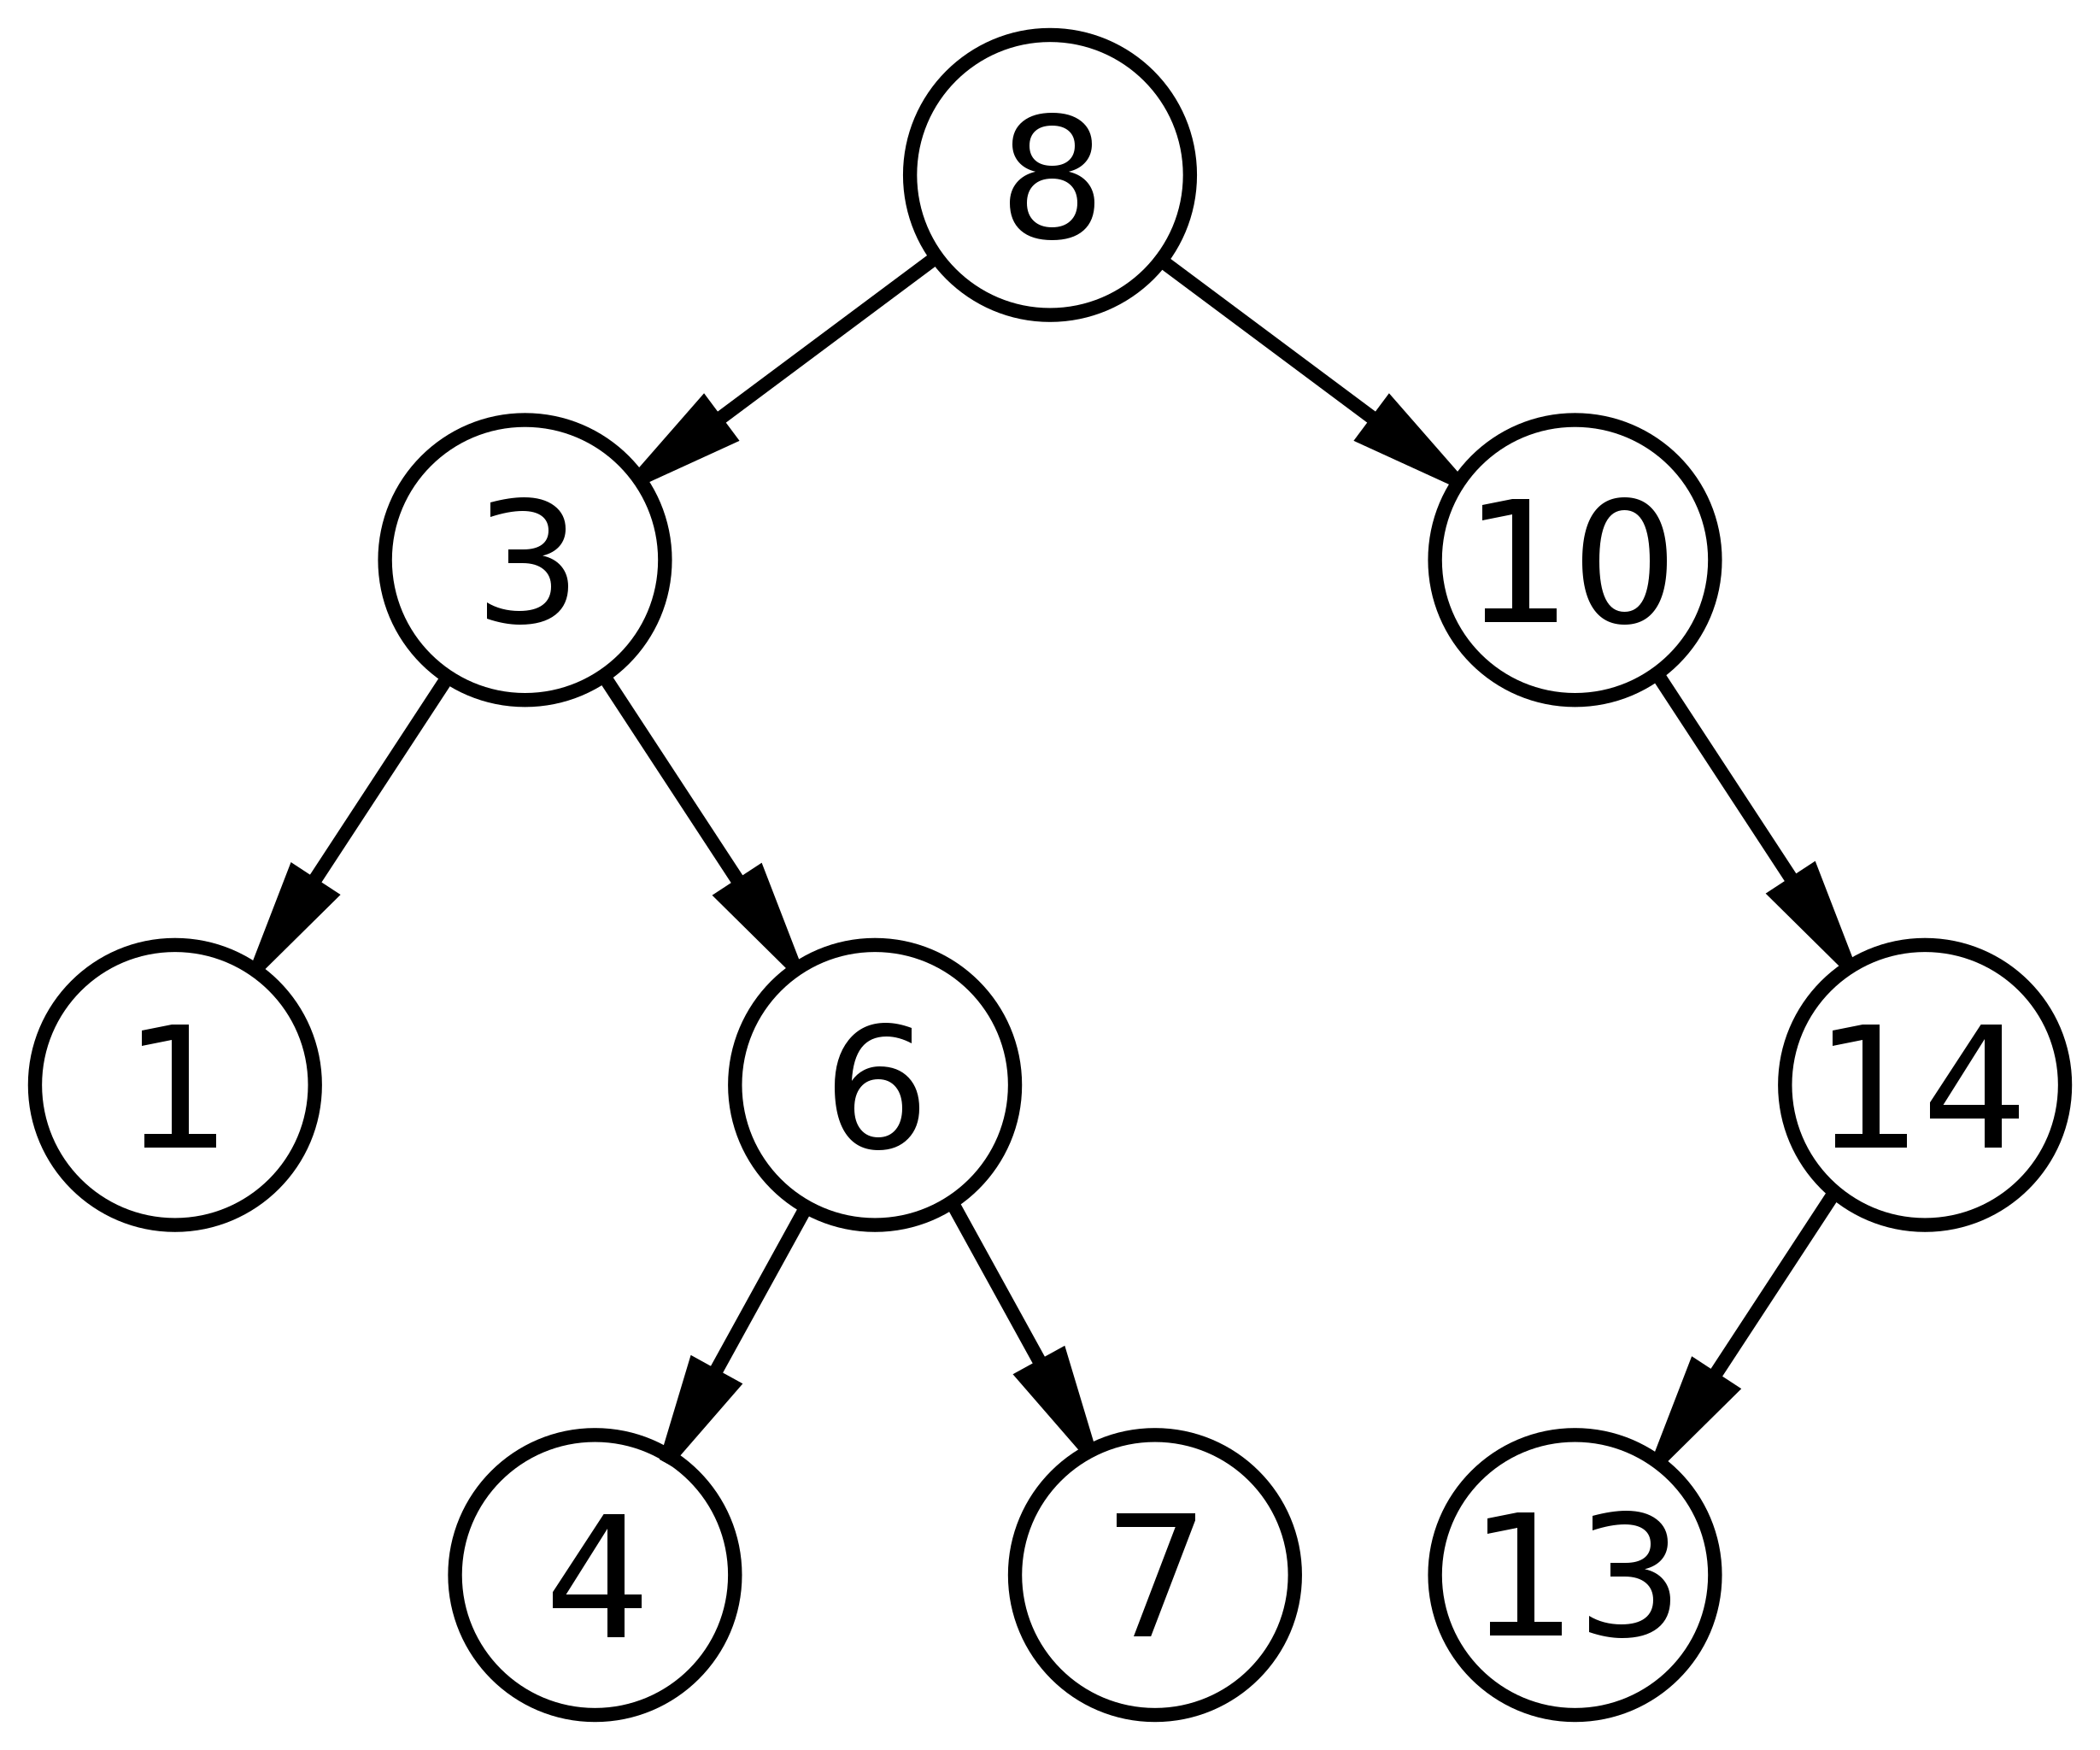
\includegraphics[width=0.25\textwidth]{BinarySearchTree}
\end{wrapfigure}Logic Theorist prechádzal cez binárny vyhľadávací strom. Koreňom stromu bola počiatočná hypotéza a každá vetva bola dedukcia založená na pravidlách logiky. Cieľom programu bolo dostať sa k výroku, ktorý sa snažil dokázať. Všetky kroky, cez ktoré program prešiel tvoria dôkaz – sériu tvrdení, ktoré viedli od hypotézy k výroku, ktorý mal dokázať.\\\textbf{Heuristika}   
\chapter{Ako sa umelá inteligencia učí}
\chapter{Umelá inteligencia a stolové hry}
Stolové hry boli súčasťou vývinu umelej inteligencie 
\chapter{Deep Blue}
\chapter{AlphaGo}
\chapter{Moderné umelé inteligencie v stolových hrách}
\bibliography{myBib}{}
\bibliographystyle{plain}
\end{document}
